\section{Inledning}

Målet med projektet har varit att konstruera ett system som kör bilar runt en
bilbana (se Figur \ref{fig:bilbanan}) på en vald referenstid mellan 12 och 15
sekunder. Syftet var att lära sig att arbeta utifrån projektstyrningsmodellen
LIPS. Systemet skulle fungera oavsett vilken av de tillhandahållna bilarna som
kördes. Ytterligare krav återfinns i kravspecifikationen och hur systemet
presterade presenteras i Appendix~\ref{app:kravbeskrivning}.

\begin{figure}
	\centering
	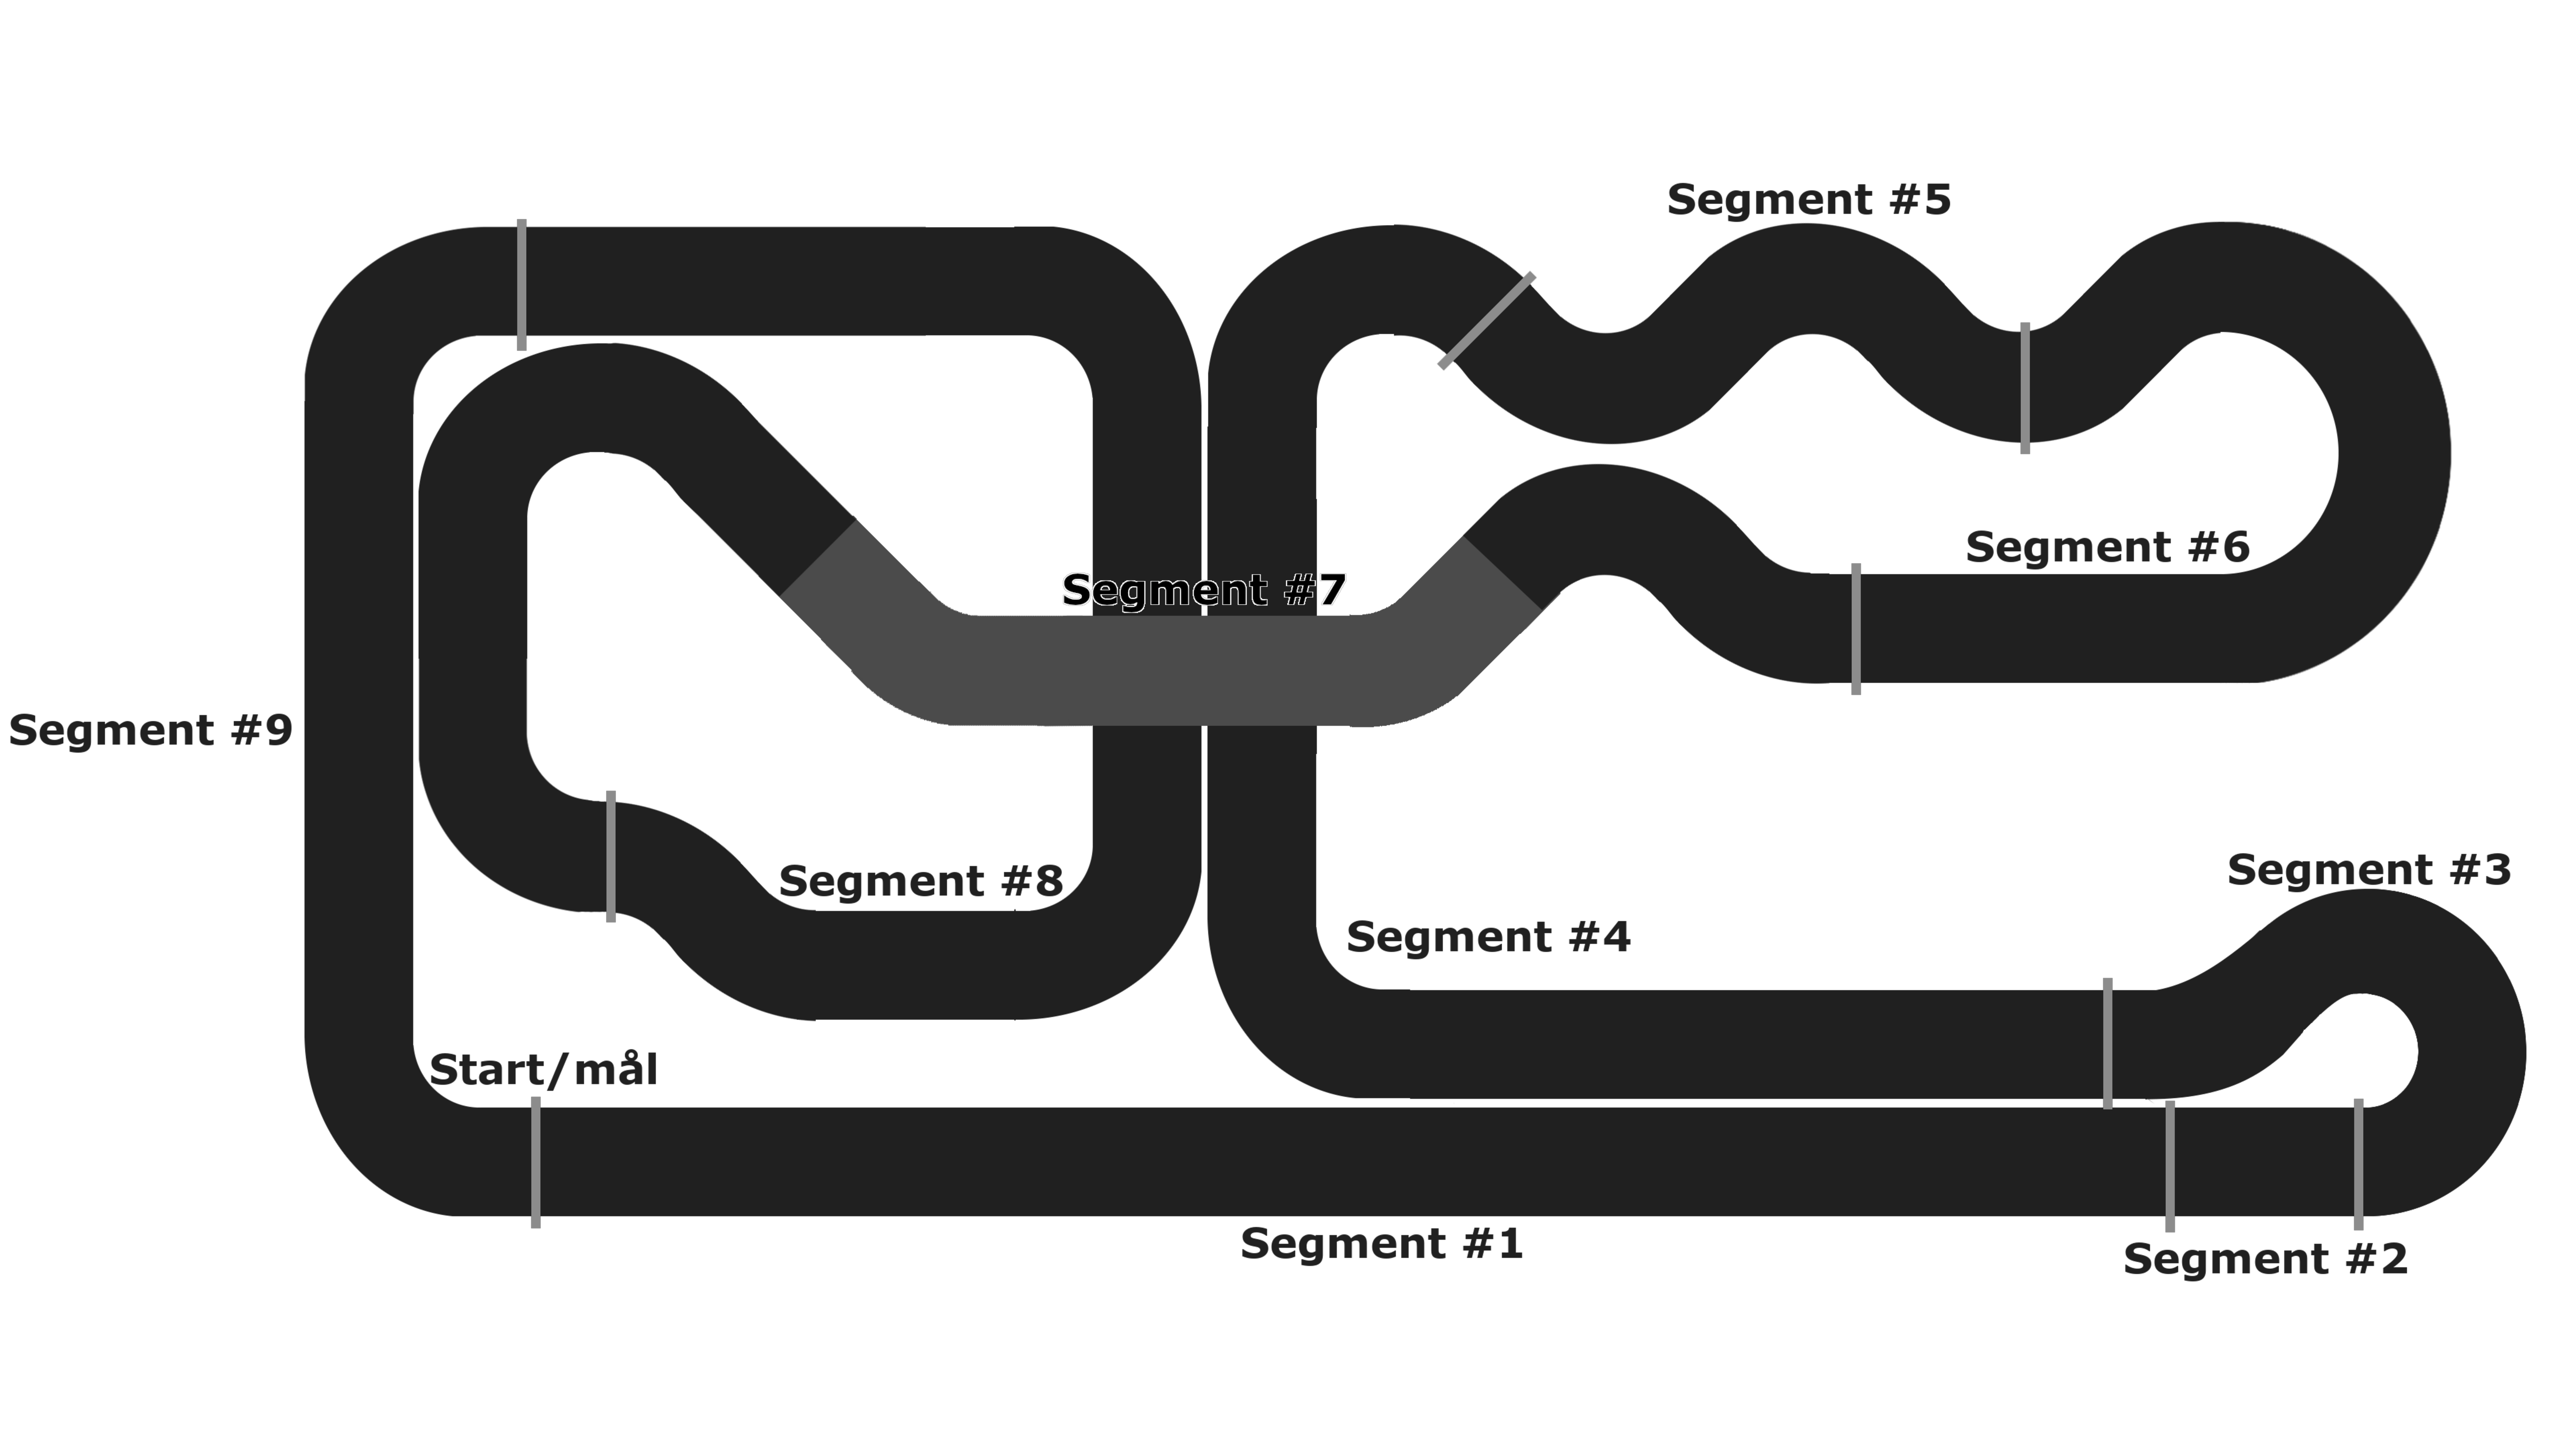
\includegraphics[width=\linewidth] {Figures/BanaModell}
	\caption{En modell av bilbanan.}
	\label{fig:bilbanan}
\end{figure} 

Projektet har utförts med
%Det material som tillhandahölls för projektet var:
en bilbana, flera bilar, givare, en extern touchdisplay, spänningsaggregat och
två datorer. Via en av datorerna har spänning tillförts bilbanan för att
kontrollera bilarnas hastighet och med hjälp av givarna har det varit möjligt
att veta när en bil varit vid en viss position.
